\documentclass[11pt,a4paper]{article}
\usepackage{amsmath,amssymb,amsthm}
\usepackage{mathtools}
\usepackage{bm}
\usepackage{booktabs}
\usepackage{array}
\usepackage{enumitem}
\usepackage{geometry}
\usepackage{graphicx}
\usepackage{subcaption}
\usepackage{xcolor}
\usepackage{tcolorbox}
\usepackage{listings}
\usepackage[pdfencoding=auto,psdextra]{hyperref}

\geometry{margin=2.5cm}
\setlength{\emergencystretch}{3em}

\newcommand{\E}{\mathbb{E}}
\newcommand{\norm}[1]{\left\lVert #1 \right\rVert}
\newcommand{\dk}{d_k}
\newcommand{\dt}{\Delta t}
\newcommand{\str}{\sigma_{\mathrm{tr}}}
\newcommand{\KL}{\mathrm{KL}}
\newcommand{\N}{\mathcal{N}}

\newtheorem*{remark*}{Remark}

\lstset{
  basicstyle=\ttfamily\small,
  breaklines=true,
  columns=fullflexible,
  keepspaces=true,
  frame=single,
  framesep=4pt,
  xleftmargin=4pt,
}

\title{\textbf{Matching the 9B teacher better makes the 4B student worse}\\[0.3em]
\large A reverse separation between the distillation objective and every reward,
reproduced across three samplers}
\author{runs \texttt{096do06e} / \texttt{gljfjziu} (2026-07-30), \texttt{ta1qvnuz} /
\texttt{z2hm869y} (2026-06)}
\date{2026-07-30}

\begin{document}
\maketitle

\begin{abstract}
Two 9B$\to$4B arms were run side by side, identical except for the P-OPD responsibility gate. At
the first scheduled eval both had reduced the held-out transition-matching loss by $18$--$21\%$ on
unseen prompts, measured on the deterministic ODE trajectories used at eval, and both had lost
reward on all three metrics: GenEval $-13\%$, OCR $-48$ to $-55\%$, PickScore $-1.5\%$. The two
arms are indistinguishable, so the gate is not the cause; the gate was also healthy, sitting at
$\gamma\approx0.62$ with only $5\%$ of transitions closed. The same regression appears in the
original dense-ODE 9B$\to$4B baseline from June, which starts at GenEval $0.376$ --- the 9B
teacher's own measured score is $0.377$ --- drops to $0.236$ at its first eval and never returns.
Distillation is working; the target is not worth reaching. Two measurements are missing before the
9B teacher can be discarded on the record: its score under the current eval configuration, and its
OCR score, which has never been measured.
\end{abstract}

\tableofcontents

%% ============================================================
\section{What was run}
\label{sec:setup}
%% ============================================================

Both of today's arms use the FLUX.2-klein-base-9B teacher into a LoRA FLUX.2-klein-base-4B
student, \texttt{Flow-SDE} at \texttt{noise\_level} $0.7$ with four trained transitions per
rollout, the covariance-normalized transition KL on \texttt{xt}, a 1:1 geneval\_enhanced$+$ocr
prompt mixture, 16 GPUs each, one optimizer step per epoch, and eval at $512$px / $40$ ODE steps
on geneval\_enhanced, ocr and pickscore at $\mathrm{gs}=1.0$. The only difference between them is
\texttt{xopd\_target\_mode}: \texttt{p\_opd} gates the teacher term by the mixture responsibility
$\gamma$ at the calibrated $T=107$, $\alpha=0.731$ (see
\texttt{popd\_exact\_sum\_gate\_saturation.tex}); \texttt{direct} does not gate at all.

Two June runs enter as historical context. \texttt{ta1qvnuz} is the original 9B$\to$4B baseline:
\texttt{ODE} with dense supervision on all 28 steps, no gate, eval at $1024$px / $28$ steps on
\texttt{dataset/geneval}. \texttt{z2hm869y} used a dense SDE (27 of 28 steps noised) and, more
importantly, evaluated the teacher itself. Absolute values are not comparable across the two eras
(different resolution, step count and GenEval variant), so the June runs are read only through
changes relative to their own epoch~0 and against the teacher measured under the same
configuration.

%% ============================================================
\section{The objective improves and the samples degrade}
\label{sec:separation}
%% ============================================================

\begin{table}[htbp]
\centering
\caption{Both arms at epoch 0 (the undistilled 4B student) and at the first scheduled eval
(epoch 100). Held-out $\dk$ is the ungated transition-matching loss on test prompts, averaged over
all 40 eval steps of the ODE trajectory: lower is a better match to the teacher. Rewards are the
three domain metrics at $\mathrm{gs}=1.0$; PickScore is logged after the division by 26 in
\texttt{rewards/pick\_score.py}.}
\label{tab:separation}
\begin{tabular}{@{}lrrr@{\hspace{2em}}rrr@{}}
\toprule
& \multicolumn{3}{c}{held-out $\dk$ (lower = closer to teacher)}
& \multicolumn{3}{c}{reward (higher = better)}\\
\cmidrule(r){2-4}\cmidrule(l){5-7}
& geneval & ocr & pickscore & GenEval & OCR & PickScore\\
\midrule
epoch 0 (base 4B) & $3.60$e-5 & $4.51$e-5 & $4.24$e-5 & $0.4559$ & $0.1486$ & $0.7570$\\
\midrule
P-OPD, epoch 100  & $2.97$e-5 & $3.67$e-5 & $3.54$e-5 & $0.3931$ & $0.0771$ & $0.7431$\\
\quad change      & $-17.6\%$ & $-18.7\%$ & $-16.4\%$ & $-13.8\%$ & $-48.1\%$ & $-1.8\%$\\
\midrule
direct, epoch 100 & $2.84$e-5 & $3.55$e-5 & $3.43$e-5 & $0.3980$ & $0.0665$ & $0.7469$\\
\quad change      & $-21.3\%$ & $-21.3\%$ & $-19.0\%$ & $-12.7\%$ & $-55.2\%$ & $-1.3\%$\\
\bottomrule
\end{tabular}
\end{table}

Table~\ref{tab:separation} is the whole finding. Three properties of the held-out $\dk$ make it
hard to dismiss as a measurement artifact:

\begin{itemize}[leftmargin=1.4em,itemsep=0.25em]
\item it is computed on \emph{test} prompts the student never trained on, so the improvement is
      generalization and not memorization;
\item it is computed on the \emph{eval} trajectories --- deterministic ODE, 40 steps --- not on the
      noisy Flow-SDE rollouts used for training, so it is not an artifact of the training
      distribution;
\item it is \emph{ungated} in both arms (\texttt{\_validation\_d\_k\_per\_timestep} calls
      \texttt{compute\_per\_step\_kl} directly), so the two arms' numbers are directly comparable
      and the gated arm cannot look better merely by multiplying its loss by $\gamma<1$.
\end{itemize}

Figure~\ref{fig:separation}(b) adds that the improvement is not concentrated anywhere: the
per-step $\dk$ profile shifts down almost in parallel across all 40 steps, and the two arms lie on
top of each other. The student is becoming more teacher-like everywhere along the trajectory that
eval actually uses, and it is getting worse at everything we measure.

\begin{figure}[htbp]
\centering
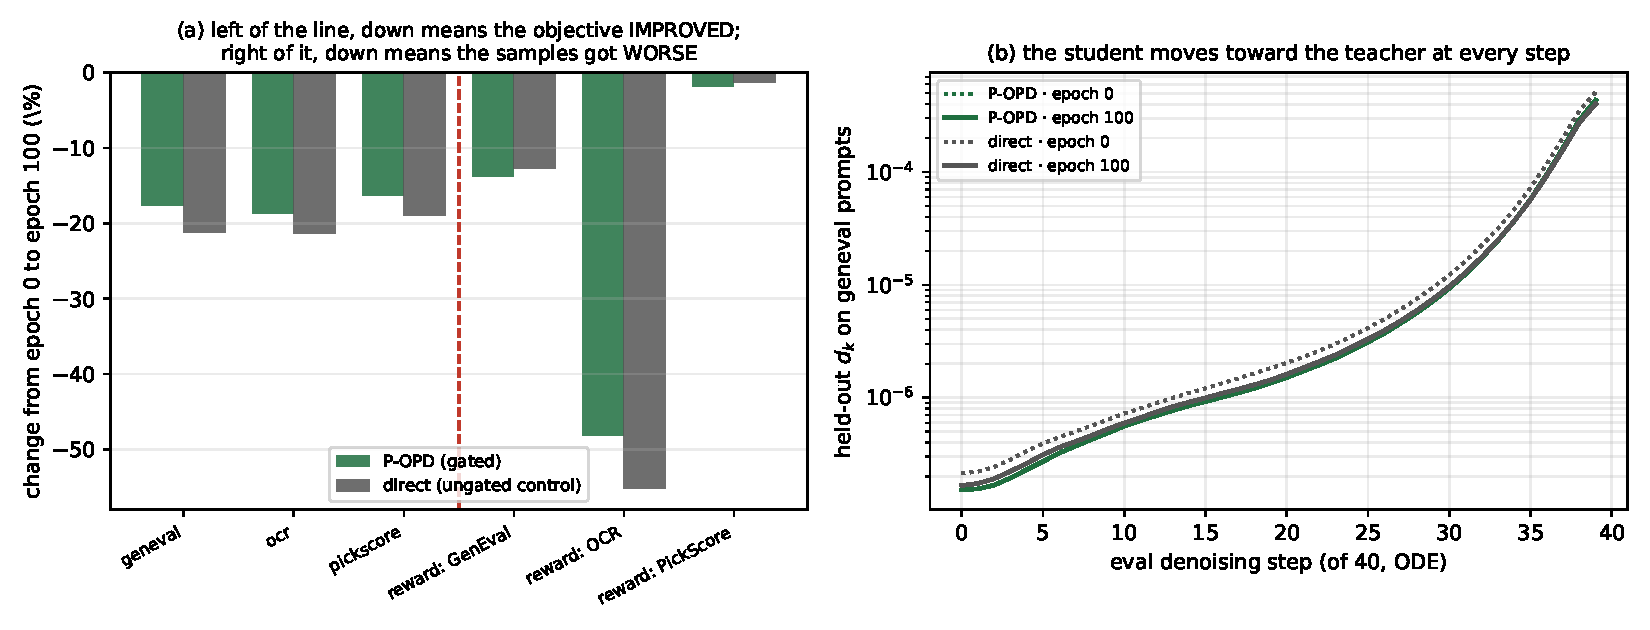
\includegraphics[width=\textwidth]{figures/9b_teacher_reverse_separation.pdf}
\caption{(a) Change from epoch 0 to epoch 100. The three bars left of the dashed line are the
held-out objective, where down is progress; the three on the right are rewards, where down is
damage. (b) Held-out $\dk$ per eval denoising step, epoch 0 (dotted) against epoch 100 (solid).
Both arms overlap, and the shift is uniform along the trajectory.}
\label{fig:separation}
\end{figure}

\subsection{The gate is exonerated, and separately shown to be inert}
\label{ssec:gate}

The ungated control reduced held-out $\dk$ \emph{more} than the gated arm ($-21.3\%$ against
$-17.6\%$ on geneval prompts) and lost a comparable amount of reward. Whatever is going wrong does
not need the gate to happen.

This also settles, negatively, the question the pair was built to answer. The gate was not
misconfigured and not saturated: over the 100 epochs $\gamma$ averaged $0.622$ with only $5.4\%$
of transitions below $0.01$, and it drifted upward from about $0.60$ to $0.70$ as $K$ fell, which
is the self-annealing behavior predicted in \texttt{popd\_exact\_sum\_gate\_saturation.tex}. A
correctly calibrated, actively varying gate changed nothing measurable. That is consistent with
the structural finding of that note --- under a single global temperature the responsibility mostly
reweights the denoising axis rather than selecting per sample --- but it cannot be a verdict on
P-OPD as a method, because a gate can only modulate how fast the student moves toward a target,
and \S\ref{sec:cause} argues this target is the problem.

%% ============================================================
\section{The same regression predates P-OPD}
\label{sec:cause}
%% ============================================================

\begin{table}[htbp]
\centering
\caption{GenEval at $\mathrm{gs}=1.0$ across three supervision regimes. The June runs are on
\texttt{dataset/geneval} at $1024$px / 28 steps; today's are on \texttt{geneval\_enhanced} at
$512$px / 40 steps, so the columns are comparable within a row-pair but not across eras. ``after''
is the first eval after training begins (epoch 20 for the June runs, 100 for today's);
\texttt{ta1qvnuz} recovers only to $0.268$ by epoch 480. The 9B teacher was measured twice under
the June configuration by two independent runs, and never under today's.}
\label{tab:three-regimes}
\begin{tabular}{@{}llrrr@{}}
\toprule
run & supervision & start & after & teacher\\
\midrule
\texttt{ta1qvnuz} (Jun 25) & ODE, dense 28/28, direct       & $0.376$ & $0.236$ & $0.377$\\
\texttt{z2hm869y} (Jun 27) & SDE, dense 27/28, $+$REINFORCE & ---     & $0.257$ & $0.377$\\
\texttt{gljfjziu} (Jul 30) & SDE, sparse 4/28, direct       & $0.456$ & $0.398$ & n/a\\
\texttt{096do06e} (Jul 30) & SDE, sparse 4/28, P-OPD gated  & $0.456$ & $0.393$ & n/a\\
\bottomrule
\end{tabular}
\end{table}

The regression reproduces under dense ODE supervision on all 28 steps, under a dense SDE on 27,
and under the sparse 4-step SDE that P-OPD requires. It is therefore a property of the 9B$\to$4B
pair and this objective, not of the sampler, the supervision density, or the gate.

The June baseline is the most informative of the four because its teacher was measured under the
identical eval configuration. Figure~\ref{fig:below} shows what happened: the untuned 4B student
began at GenEval $0.376$, statistically the same as the 9B teacher's $0.377$ --- there was nothing
to distill --- and 20 epochs of teacher matching moved it to $0.236$. Over the next 460 epochs it
recovered only to $0.268$, still well below where it started.

\begin{figure}[htbp]
\centering
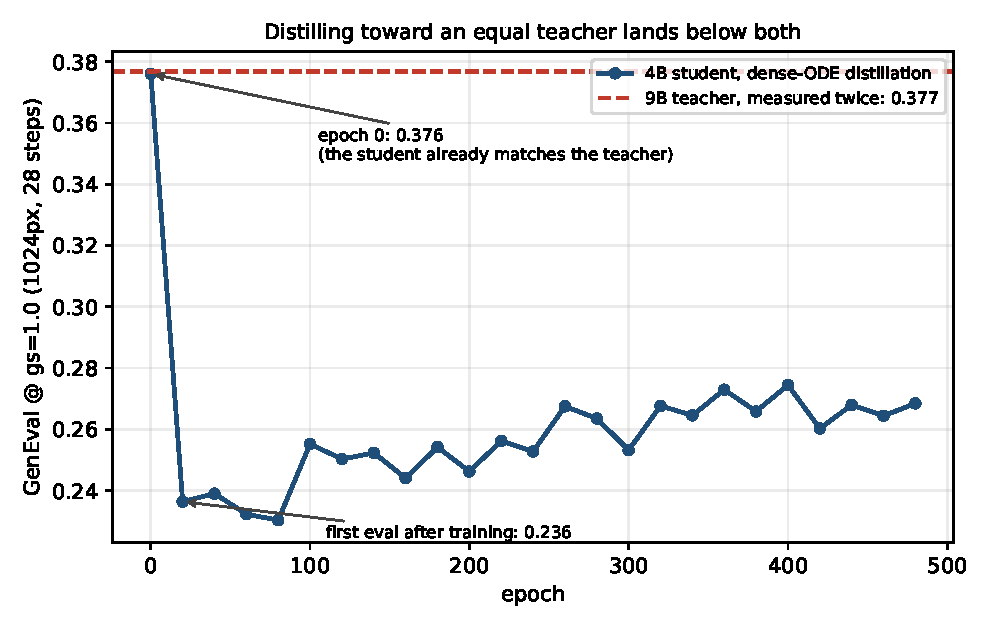
\includegraphics[width=0.78\textwidth]{figures/9b_teacher_below_both.pdf}
\caption{The original dense-ODE 9B$\to$4B baseline (\texttt{ta1qvnuz}). The student starts level
with the teacher, drops sharply, and settles below both. The teacher line is the mean of two
independent measurements ($0.3773$, $0.3762$) taken under the same eval configuration.}
\label{fig:below}
\end{figure}

\subsection{A matched 32B control changes only the target and reverses the result}
\label{ssec:matched-32b}

The historical run \texttt{4wvzbt8g} is the missing control. It uses the 32B FLUX.2-dev teacher,
but otherwise matches \texttt{ta1qvnuz}: the same base 4B student, seed 42, Geneval prompts,
512px training, a dense 28-step ODE, direct transition-mean matching, LoRA rank 64 with
$\alpha=128$, learning rate $10^{-4}$, EMA 0.9, 128 unique prompts and one optimizer update per
epoch, and 1024px/28-step evaluation at guidance scales 1 and 4. The 32B teacher requires batch
size 1 instead of 4 and gradient checkpointing, but gradient accumulation preserves the same
128-prompt update. The runs used commits one day apart; the trainer change precomputes and
offloads teacher text embeddings and does not alter the objective.

\begin{table}[htbp]
\centering
\caption{The controlled ODE pair through their common epoch-80 window. Both losses decrease.
The rewards move in opposite directions. Absolute $\dk$ values are not compared across teachers,
because each teacher defines a different target gap.}
\label{tab:matched-ode}
\begin{tabular}{@{}lrrr@{\hspace{1.3em}}rrr@{}}
\toprule
& \multicolumn{3}{c}{$\dk$ (lower is closer)}
& \multicolumn{3}{c}{GenEval reward (higher is better)}\\
\cmidrule(r){2-4}\cmidrule(l){5-7}
teacher & epoch 0 & epoch 80 & change
& gs & epoch 0 & epoch 80 (change)\\
\midrule
9B  & $8.368$e-5 & $7.071$e-5 & $-15.5\%$
    & 1 & $0.3760$ & $0.2303$ ($-38.7\%$)\\
    &             &             &
    & 4 & $0.7507$ & $0.6877$ ($-8.4\%$)\\
\midrule
32B & $2.170$e-4 & $1.596$e-4 & $-26.5\%$
    & 1 & $0.3760$ & $0.7772$ ($+106.7\%$)\\
    &             &             &
    & 4 & $0.7507$ & $0.8093$ ($+7.8\%$)\\
\bottomrule
\end{tabular}
\end{table}

\begin{figure}[htbp]
\centering
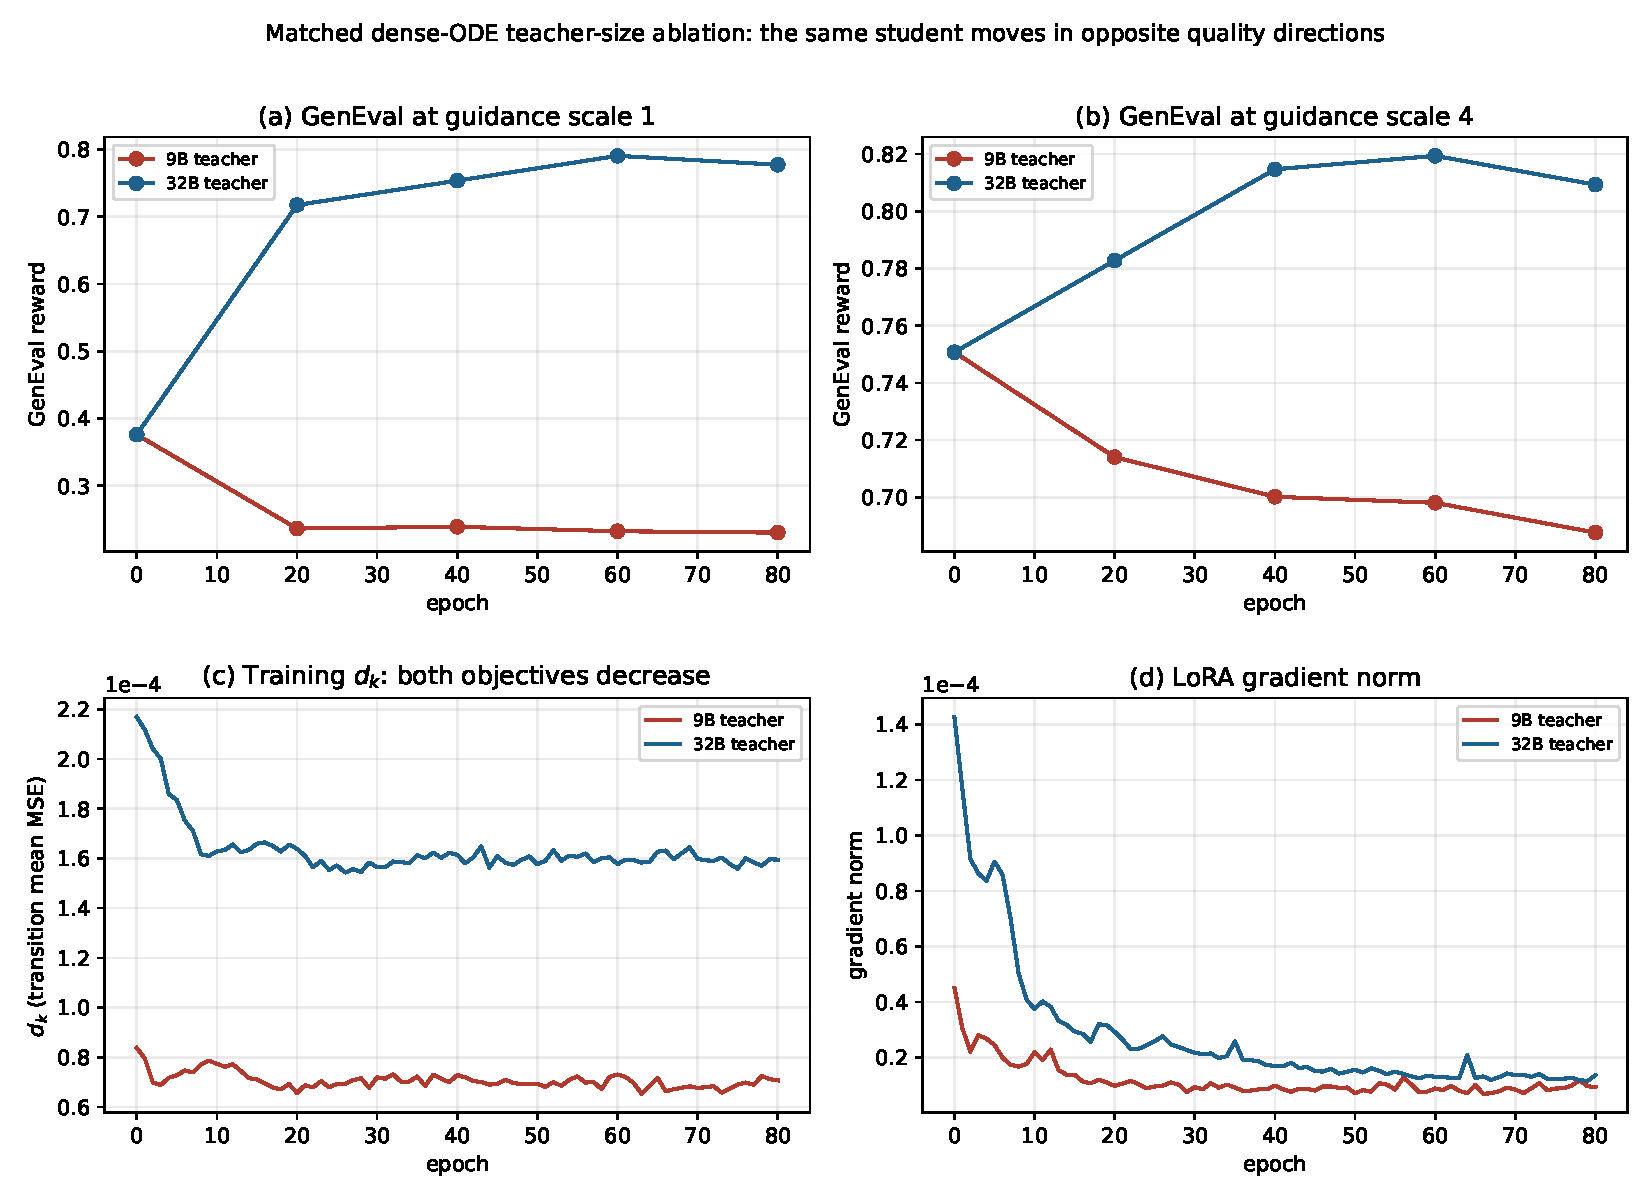
\includegraphics[width=\textwidth]{figures/ode_9b_vs_32b_matched.pdf}
\caption{The matched teacher-size ablation. Both arms begin from exactly the same student reward
and both reduce their own transition-matching loss. Only the teacher changes, and the quality
direction reverses.}
\label{fig:matched-ode}
\end{figure}

The fixed 18-image panels at each guidance scale give the same answer without using the reward
model. We pair every prompt and seed, embed all images with CLIP and DINOv2, and measure LPIPS
against the common epoch-0 base. At epoch 80 the 32B arm has moved \emph{farther}: LPIPS is
$0.605$ against $0.294$ for the 9B arm, CLIP cosine to the base is $0.802$ against $0.889$, and
DINOv2 cosine is $0.564$ against $0.702$. In 10,000 paired bootstrap resamples, the
32B-minus-9B LPIPS difference is $0.311$ with 95\% CI $[0.246,0.373]$; the CLIP-cosine difference
is $-0.087$ with CI $[-0.134,-0.041]$, and the DINOv2 difference is $-0.138$ with CI
$[-0.229,-0.051]$. All three reject equal movement.

\begin{figure}[htbp]
\centering
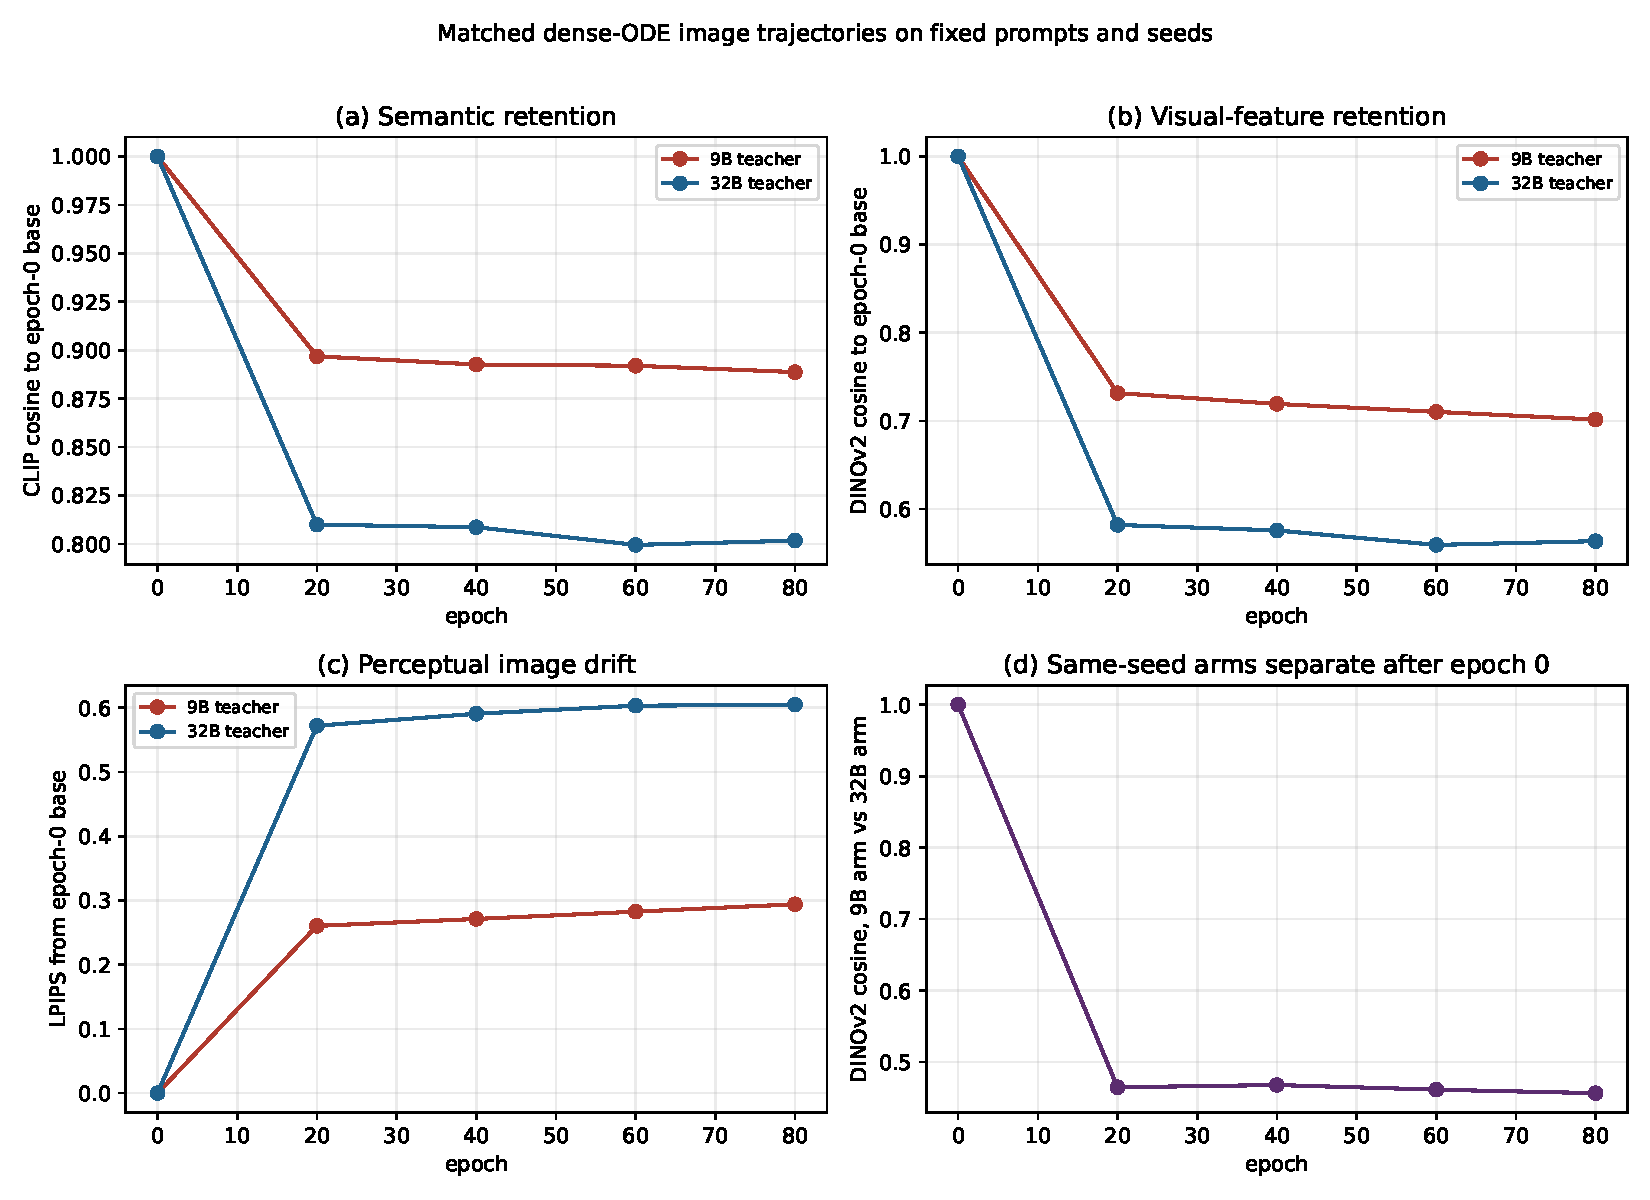
\includegraphics[width=\textwidth]{figures/ode_9b_vs_32b_image_drift.pdf}
\caption{Image drift from the identical epoch-0 4B student on fixed prompts and seeds. The useful
32B update is substantially larger than the harmful 9B update. Update magnitude alone cannot
explain the regression.}
\label{fig:image-drift}
\end{figure}

The phenomenon and conclusion are simple. The 9B arm moves less and gets worse. The 32B arm moves
more and gets better. Therefore a trust region that only caps update size is not the missing
ingredient. It can slow either direction, but cannot tell a useful teacher direction from a
harmful one.

\begin{tcolorbox}[colback=red!4!white,colframe=red!45!black,title={The student lands below BOTH endpoints, which is stronger than
``the teacher is worse''}]
If the teacher merely scored lower, matching it should walk the student down \emph{toward} the
teacher's score and stop there. Instead the student ends at $0.236$--$0.268$ against two endpoints
at $\approx0.377$. Partially matching another model's transition means does not interpolate
quality: the LoRA lands on a velocity field that is neither the student's nor the teacher's and is
worse than both.

The same effect was measured this morning on a different question. The MoF-2 checkpoint routes
every prompt to a 50/50 blend of two experts; on OCR that blend scores $0.6313$ against $0.6314$
and $0.6476$ for the experts alone, i.e.\ below the mean of the two and level with the weaker one
(\texttt{/root/router\_viz/SUMMARY.md}). Averaging two velocity fields destroyed a capability that
both of its endpoints partly had. A blend and a partial distillation move are the same operation
on the velocity field, and both are worse than they look.
\end{tcolorbox}

\begin{remark*}
The matched pair isolates the teacher, but not the damaging property of its velocity field. The
remaining questions are local: whether the checkpoint update aligns with the teacher residual,
whether only specific denoising steps are harmful, and whether the 9B and 32B residuals occupy
different low-rank directions. The checkpoint probe in the next revision measures these quantities
on the same base-student states, so on-policy state drift cannot confound the comparison.
\end{remark*}

%% ============================================================
\section{What is not yet measured}
\label{sec:gaps}
%% ============================================================

\begin{enumerate}[leftmargin=1.6em,itemsep=0.3em]
\item \textbf{The 9B teacher under the current eval configuration.} Its $0.377$ was measured at
      $1024$px / 28 steps on \texttt{dataset/geneval}; today's students are scored at $512$px / 40
      steps on \texttt{geneval\_enhanced}, where the base 4B reads $0.456$. Until the teacher is
      scored the same way, ``the teacher is no better than the student'' is an inference from a
      cross-configuration comparison, not a measurement. \texttt{eval\_teacher\_at\_start: true}
      on either arm's config answers it in roughly 40 minutes on 32 GPUs.
\item \textbf{The teacher's OCR score, which has never been measured at all.} OCR is where the
      damage is worst ($-48\%$ / $-55\%$) and where the base student is weakest ($0.1486$), and no
      run has ever evaluated the 9B teacher on it.
\item \textbf{Whether the loss space is a co-cause.} A \texttt{direct} arm on the ODE sampler with
      \texttt{xopd\_dk\_space: v} and \texttt{normalize\_d\_k: false} --- the configuration the
      32B$\to$4B runs improve under --- would separate ``9B is a bad teacher'' from ``this loss
      space is a bad objective''.
\end{enumerate}

\begin{tcolorbox}[colback=blue!3!white,colframe=blue!40!black,title={Consequence for the P-OPD programme}]
P-OPD cannot be evaluated on 9B$\to$4B. A gate that suppresses implausible teacher transitions can
at best slow a descent toward a target that should not be reached; the honest test needs a teacher
whose ungated baseline improves the student, which on this cluster means FLUX.2-dev at 32B.
\end{tcolorbox}

%% ============================================================
\section*{Reproducing}
\addcontentsline{toc}{section}{Reproducing}
%% ============================================================

\begin{lstlisting}[language=bash]
# figures and the cached numbers used in this note
python scripts/xopd_analysis/plot_9b_teacher_regression.py

# the two arms (16 GPUs each; identical except xopd_target_mode)
XOPD_WORKERS="28.7.185.215" MASTER_PORT=29650 bash scripts/xopd_cluster/run_4node_xopd.sh \
  xopd_configs/sde_pathwise/flux2_klein_9b_to_4b_popd_mix_1kep.yaml
XOPD_WORKERS="28.7.195.15" MASTER_IP=28.7.185.156 MASTER_PORT=29660 \
  bash scripts/xopd_cluster/run_4node_xopd.sh \
  xopd_configs/sde_pathwise/flux2_klein_9b_to_4b_direct_ctrl_mix_1kep.yaml
\end{lstlisting}

Cached numbers: \path{docs/xopd/diagnostics/figures/9b_teacher_regression.json}.
Gate calibration and per-step structure:
\path{docs/xopd/core/p_opd/popd_exact_sum_gate_saturation.tex}.
Per-step loss weighting theory:
\path{docs/xopd/core/shared/per_timestep_loss_dominance_theory.tex}.

\end{document}
